% Unofficial University of Cambridge Poster Template
% https://github.com/andiac/gemini-cam
% a fork of https://github.com/anishathalye/gemini
% also refer to https://github.com/k4rtik/uchicago-poster

\documentclass[final]{beamer}

% ====================
% Packages
% ====================

\usepackage[T1]{fontenc}
\usepackage{lmodern}
\usepackage[orientation=portrait,size=a2,scale=1.15]{beamerposter}
\usetheme{gemini}
\usecolortheme{nott}
\usepackage{graphicx}
\usepackage{booktabs}
\usepackage{tikz}
\usepackage{pgfplots}
\pgfplotsset{compat=1.14}
\usepackage{anyfontsize}
\usepackage[absolute,overlay]{textpos}
\setlength{\TPHorizModule}{1cm}
\setlength{\TPVertModule}{1cm}
\textblockorigin{0cm}{0cm}  % 设
\usepackage[most]{tcolorbox}
\usepackage{xcolor}
\usepackage{fontawesome5}
% ====================
% Lengths
% ====================

% If you have N columns, choose \sepwidth and \colwidth such that
% (N+1)*\sepwidth + N*\colwidth = \paperwidth
\newlength{\sepwidth}
\newlength{\colwidth}
\setlength{\sepwidth}{0.025\paperwidth}
\setlength{\colwidth}{0.45\paperwidth}

\newcommand{\separatorcolumn}{\begin{column}{\sepwidth}\end{column}}

% ====================
% Title
% ====================

\title{On the importance of tail assumptions in climate extreme event attribution}

\author{Mengran Li,\and Daniela Castro-Camilo }
\institute{School of Mathematics and Statistics, University of Glasgow, UK}

% ====================
% Footer (optional)
% ====================

\footercontent{
  65th ISI World Statistics Congress, The Hague, 2025 \hfill
  \href{mailto:m.li.3@research.gla.ac.uk}{m.li.3@research.gla.ac.uk}}
% (can be left out to remove footer)


% ====================
% Logo (optional)
% ====================

% use this to include logos on the left and/or right side of the header:
%\logoright{
\includegraphics[height=2.2cm]{logos/UoG_keyline.png}}
%\logoleft{
\includegraphics[height=2.2cm]{logos/UoG_keyline.png}}


\definecolor{headlinebg}{RGB}{0,51,89}
\setbeamercolor{headline}{fg=white, bg=headlinebg}
% ====================
% Body
% ====================

\begin{document}

\addtobeamertemplate{headline}{}{
  \begin{tikzpicture}[remember picture,overlay]
    % 假设标题栏高度约为 6ex,上下偏移调节 logo 到左下角
    \node[anchor=south west, inner sep=0.3cm] 
      at ([xshift=1.5cm,yshift=-45.5ex]current page.north west)
      {
\includegraphics[height=2cm]{logos/UoG_keyline.png}};
  \end{tikzpicture}
}


\begin{frame}[t]
\begin{columns}[t]
\separatorcolumn

\begin{column}{\colwidth}

  \begin{block}{Introduction}
  \textbf{Extreme event attribution (EEA)} assesses how much human-induced climate change has influenced specific extreme weather events.
As these events become more frequent and intense, robust statistical tools are essential.
We compare three multivariate models—under Pearl’s counterfactual framework—to estimate \textbf{attribution ratios (ARs)}, which quantify the probability that human influence was necessary for the event.
Model choice is critical: it must accurately capture \textbf{joint tail behaviour} in high-dimensional climate data.

\begin{tcolorbox}[colback=cyan!10!white, colframe=cyan!40!black, boxrule=0.5pt, width=18.5cm]
\begin{center}
    \textbf{\Large{Goals}}
\end{center}
1) Show how the choice of tail model in EEA affects causal attribution results\\
2) Offer practical guidance for selecting appropriate tail models in this context
\end{tcolorbox}

\end{block}


\begin{alertblock}{Extreme event attribution}
Let $E$ be the extreme event of interest, defined as 
$$\hspace{5cm}
\boxed{
E = \{ \pmb{w}^\top \pmb{X} > v \},
}\leftarrow
% \quad
\parbox{7cm}{\textcolor{red}{\small \textbf{Event occurs when a weighted climate index exceeds a high threshold \(v\)}}}
$$
where \(\pmb{X} = (X_1, \ldots, X_d)^\top\) is a climate index vector over \(d\) locations and \(\pmb{w}\) are nonnegative weights.
We estimate the probability of $E$ under two scenarios:
\[
p_i =  \mathbb{P}(E^{(i)})= \mathbb{P}[\pmb{w}^\top \pmb{X}^{(i)} > v], \quad i \in \{0,1\},
\]
where 
\begin{itemize}
    \item $\pmb{X}^{(1)}$: factual world (with human influence) $\rightarrow$ probability \textcolor{blue!70!black}{\textbf{\( p_1 \)}}
    \item $\pmb{X}^{(0)}$: factual world (without human influence) $\rightarrow$ probability \textcolor{orange!90!black}{\textbf{\( p_0 \)}}
\end{itemize}
\vspace{0.5em}
We summarise the effect of human influence via the attribution ratio (AR): 
$$
\mathrm{AR} = \frac{p_0 - p_1}{p_1} 
\leftarrow
\parbox{10cm}{Fraction of the risk attributable to human influence}
$$
\colorbox{cyan!10}{%
  \parbox{0.97\linewidth}{
  \textbf{Interpretation:}  
  An AR of 1 means the event is \textbf{twice as likely} due to human influence.  
  Higher ARs indicate stronger attribution.
  }
}
  \end{alertblock}
\vspace{-.3cm}
 \begin{block}{Methodology}
\vspace{-.3cm}
\heading{\faIcon{exclamation-triangle}\ What’s the challenge?}

\textcolor{black!80}{
Extreme events are rare and their joint behaviour across locations is complex. We compare three flexible multivariate models that capture tail dependence differently.
}
\vspace{-.3cm}
\heading{\faChartLine\ Multivariate Generalized Pareto (mGPD)}
\vspace{-.3cm}
\begin{itemize}
  \item Tail model arising from a peaks-over-threshold framework.
  \item Uses transformation of exponential and arbitrary random vectors:
  \[
  \pmb{Z}^* \overset{d}{=} E+\pmb{T}-\max_j T_j
  \quad \Rightarrow \quad
  \pmb{Z} = \frac{\pmb{\sigma}}{\pmb{\gamma}} \left( \exp(\pmb{\gamma Z}^*) - 1 \right)
  \]
  \item Has a rigid extremal dependence structure.
\end{itemize}

\vspace{-.3cm}
\heading{\faProjectDiagram\ Exponential Factor Copula Model (eFCM)}
\vspace{-.3cm}
\begin{itemize}
  \item A simple \textbf{latent factor model}: $W(s) = Z(s) + V$
  \item \(Z(s)\): Gaussian process with exponential correlation;  
        \(V \sim \exp(\lambda)\): shared random factor across space.
  \item Generates flexible tail dependence via mixing.
\end{itemize}

\vspace{-.3cm}
\heading{\faNetworkWired\ Huser & Wadsworth (HW) Model}
\vspace{-.3cm}
\begin{itemize}
  \item Blends a Gaussian process with a Pareto variable: $X(\pmb{s}) = R^{\delta} W(\pmb{s})^{1-\delta}$
  \item Parameter \(\delta\) controls \textbf{extremal dependence}:
  
  \textbullet\hspace{.5em} \(\delta > 0.5\): asymptotic dependence \hspace{1cm} \textbullet\hspace{.5em} \(\delta < 0.5\): asymptotic independence
\end{itemize}

\vspace{-.3cm}
\heading{\faSlidersH\ How do the models differ? \quad \textit{(Focus: Extremal Dependence)}}

\noindent
\begin{minipage}[t]{0.4\linewidth}
  \vspace{-.5cm}
  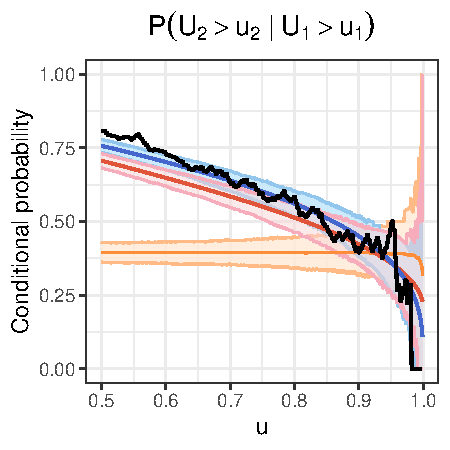
\includegraphics[width=\linewidth]{Figures/chi_poster.pdf}
\end{minipage}%
\hfill
\begin{minipage}[t]{0.55\linewidth}
  \vspace{0pt}
  \normalsize
  \textbf{What are we looking at?}  
  \\
  The strength of \textbf{conditional dependence} between the \textbf{two yellow locations} on the map, under the \textbf{counterfactual scenario}.
  \\[1ex]
  \textbf{How is it measured?}  
  \\
  Data from each location are transformed to a {uniform scale} (\(U_1, U_2\)) using their empirical distributions. We estimate the conditional probability \( \mathbb{P}(U_2 > u \mid U_1 > u) \) as \(u \to 1\)—\textbf{a key measure of tail dependence}.
  \\[1ex]
\end{minipage}

 \textbf{What does the plot show?}  \\
  \textbf{Black line} is the empirical estimator, \textbf{\textcolor{red}{red line}} is eFCM, \textbf{\textcolor{blue}{blue line}} is HW, and the \textbf{\textcolor{orange}{orange line}} is mGPD. Shaded areas show 95\% confidence intervals. \textbf{The models differ substantially in how well they capture tail dependence—crucial for reliable attribution.}

  \end{block}

\end{column}
  
\separatorcolumn

\begin{column}{\colwidth}

    \begin{block}{Simulation Study}
\vspace{-0.3cm}
\heading{\faBalanceScale\ Impact of Model Misspecification}

We simulate data from the HW model to estimate \( p = \mathbb{P}(E) \). When the \textbf{dependence structure is misspecified}, bias in \(\hat{p}\) becomes substantial—especially under strong extremal dependence. 

\textbf{Correct margins alone are not enough}; realistic dependence modelling is critical.

\begin{figure}
  \centering
  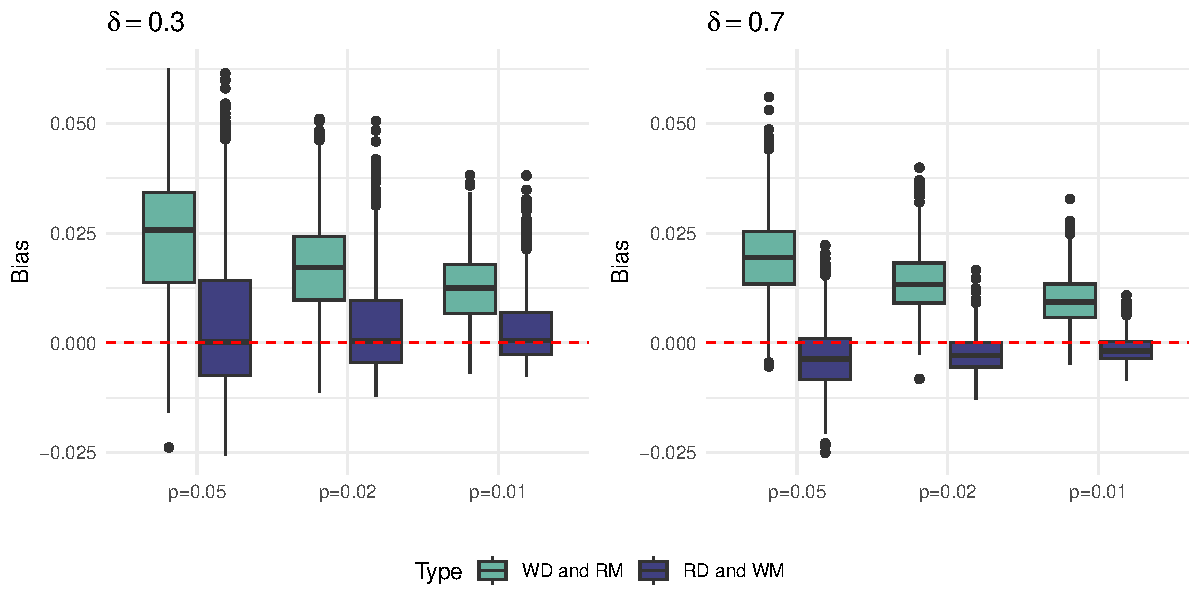
\includegraphics[width=0.8\linewidth]{Figures/simu1_boxplot.pdf}
\end{figure}

\vspace{-5pt}
\textcolor{purple}{Purple:} wrong dependence, right margins. \quad  
\textcolor{green!60!black}{Green:} right dependence, wrong margins.

\vspace{-0.1cm}
\heading{\faChartBar\ Dependence Strength Matters}

We vary extremal dependence in HW-generated data (\(\delta \in [0.3, 0.8]\)) and assess how well mGPD and eFCM recover the true tail probability.

\vspace{0.3em}
\textbf{Takeaway:} \textbf{eFCM consistently achieves lower RMSE} than mGPD across all scenarios. The gap grows as \(\delta\) increases.

\begin{center}
\scriptsize
\renewcommand{\arraystretch}{1.1}
\begin{tabular}{l c|ccccc}
      & & \multicolumn{5}{c}{$\delta$ (dependence)} \\
      Model & $p$ & 0.3 & 0.4 & 0.6 & 0.7 & 0.8 \\
      \toprule
      eFCM & 0.05 & \textbf{0.0017} & \textbf{0.0012} & \textbf{0.0008} & \textbf{0.0007} & \textbf{0.0007} \\
      mGPD &      & 0.0049 & 0.0043 & 0.0036 & 0.0035 & 0.0038 \\
      \midrule
      eFCM & 0.02 & \textbf{0.0008} & \textbf{0.0006} & \textbf{0.0005} & \textbf{0.0004} & \textbf{0.0004} \\
      mGPD &      & 0.0030 & 0.0031 & 0.0027 & 0.0026 & 0.0025 \\
      \midrule
      eFCM & 0.01 & \textbf{0.0005} & \textbf{0.0004} & \textbf{0.0003} & \textbf{0.0003} & \textbf{0.0003} \\
      mGPD &      & 0.0025 & 0.0024 & 0.0021 & 0.0022 & 0.0022 \\
\bottomrule
\end{tabular}
\end{center}

\end{block}

\vspace{-0.5cm}
\begin{block}{Precipitation Attribution: Europe and USA}

\begin{figure}
  \centering
  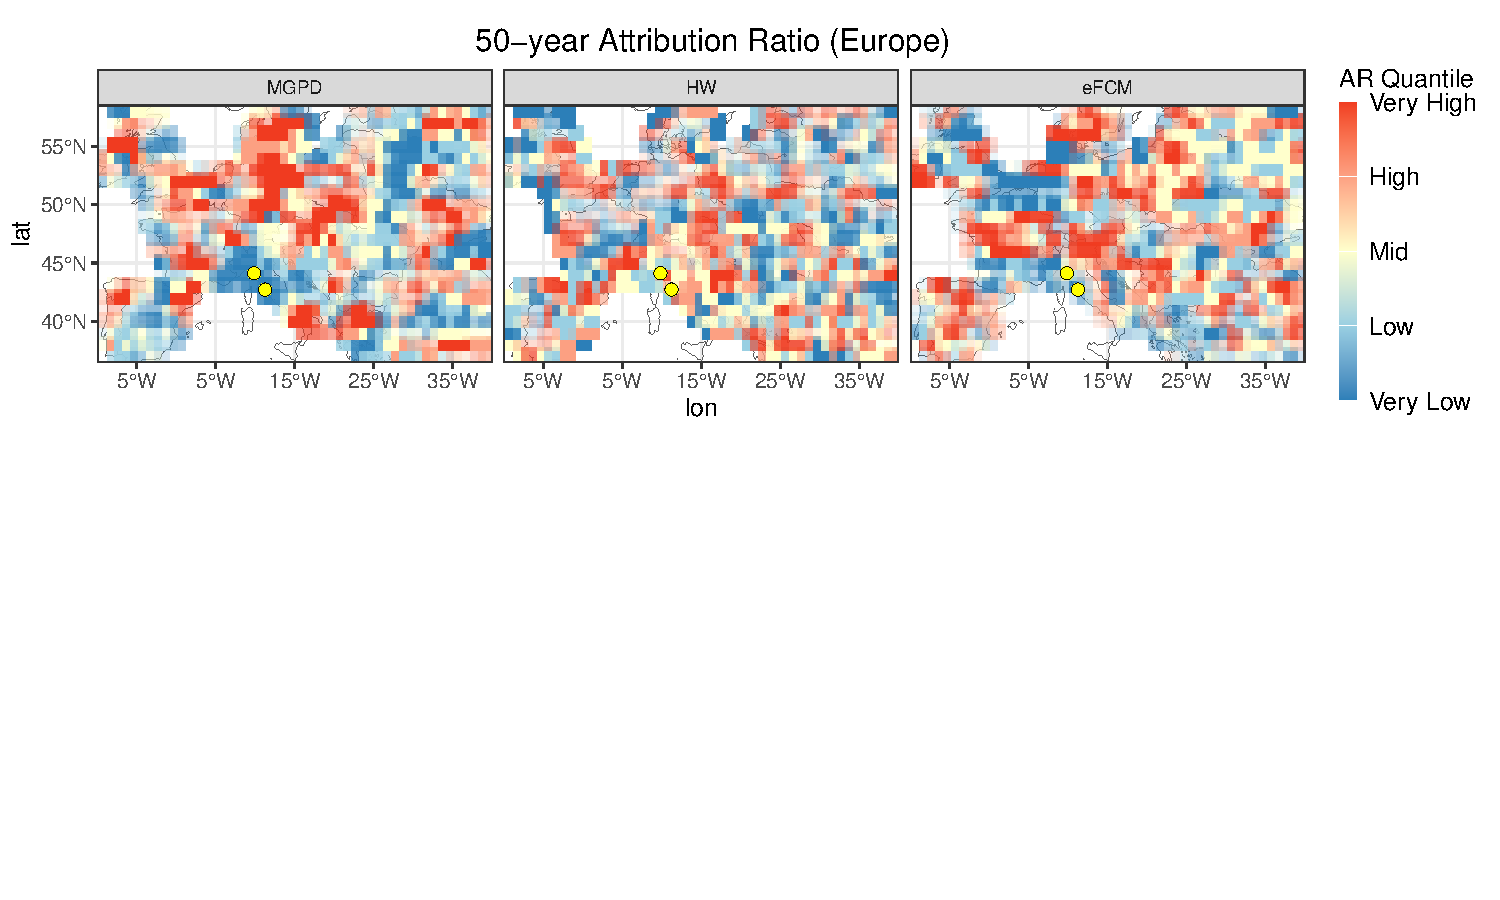
\includegraphics[width=\linewidth]{Figures/poster_map-eu.pdf}
  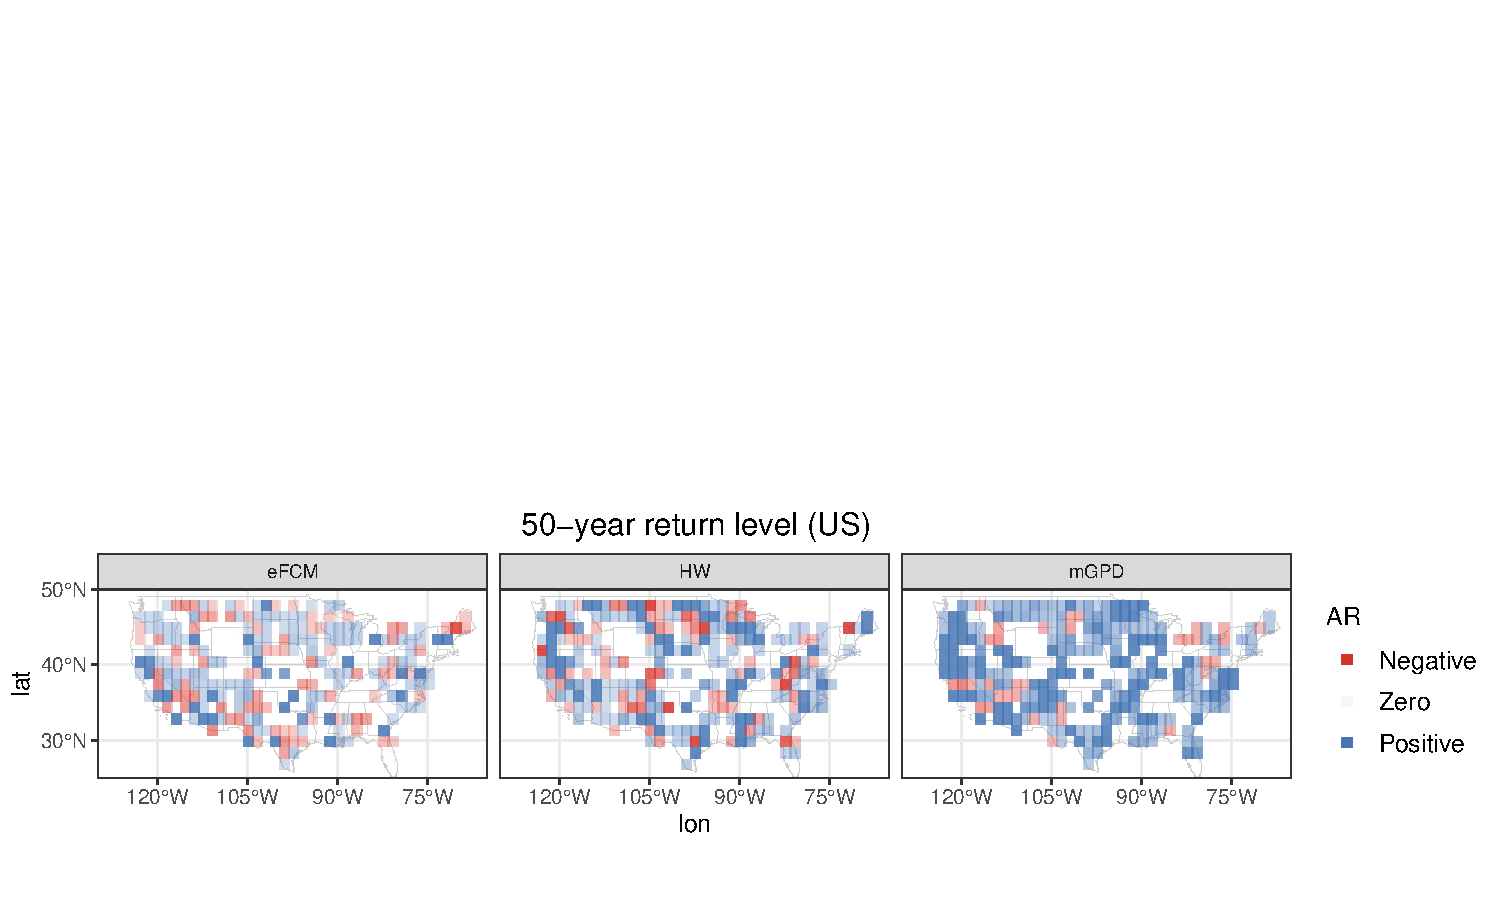
\includegraphics[width=\linewidth]{Figures/poster_map-us.pdf}
\end{figure}

\vspace{-15pt}
\textbf{Top row (Europe):} Attribution Ratios (ARs) over grid cells—blue (low AR) to red (high AR). Yellow markers show locations used in tail dependence analysis.

\textbf{Bottom row (US):} AR classification map: \textcolor{red}{red} (negative), \textcolor{gray}{white} (neutral), and \textcolor{blue}{blue} (positive).

\vspace{-0.5cm}
\begin{center}
\colorbox{cyan!10}{%
  \parbox{0.7\linewidth}{%
    \centering
    \faIcon{hand-point-right} \textbf{Model choice strongly influences spatial AR patterns}
  }
}
\end{center}


\end{block}
\vspace{-0.6cm}
\begin{block}{Conclusion}
\small
\textbullet\hspace{0.1cm}Tail model choice has a substantial effect on causal attribution estimates. \textbf{eFCM and HW} better match empirical tail dependence, while \textbf{mGPD} often overstates ARs.

\textbullet\hspace{0.1cm}\textbf{eFCM} performs best: it achieves the narrowest CIs and lowest RMSE across all simulations.

\textbullet\hspace{0.1cm}\textit{Choosing the right extremal dependence model is essential for credible EEA.}

\end{block}


\vspace{-1cm}
\begin{minipage}[t]{0.7\linewidth}
\begin{block}{\faLightbulb\ Tail Model Selection: Practical Tips}

\footnotesize

\textbf{1. Prioritise dependence structure.}  
Attribution relies on joint tail behaviour—eFCM and HW outperform mGPD under strong dependence. Conditional probability plots are a useful diagnostic.

\textbf{2. Do not trust margins alone.}  
Correct univariate fit can still yield poor ARs if dependence is misspecified.

\textbf{3. Prefer robust models.}  
eFCM offers lower RMSE and tighter intervals—strong candidate when uncertainty is high.

\vspace{0.3em}
\textbf{4. Choose interpretability.}  
HW’s \(\delta\) parameter offers intuitive insight into tail dependence strength.

\end{block}
\vspace{-0.4cm}
\begin{block}{\faIcon{code-branch} Reproducibility}

Ongoing work.
\textbf{Data and code will be made publicly available}—check back soon at:  
\url{https://your-link-here.com}

\end{block}

\end{minipage}
\hfill
\begin{minipage}[t]{0.28\linewidth}
\begin{block}{Reference Output}
\faIcon{arrow-down} Scan the QR code for references.
\vspace{10pt}
\begin{center}

\includegraphics[width=0.7\linewidth]{Figures/qr.png}
\end{center}
\end{block}

\end{minipage}


\end{column}
\separatorcolumn

\end{columns}
\end{frame}

\end{document}
